\documentclass[letterpaper, reqno,11pt]{article}
\usepackage[margin=1.0in]{geometry}
\usepackage{color,latexsym,amsmath,amssymb,graphicx,float,listings,tikz}
\usepackage{hyperref}

\hypersetup{
colorlinks=true,
linkcolor=magenta,
filecolor=magenta,
urlcolor=cyan,
}

\graphicspath{ {images/} }

\begin{document}
\pagenumbering{arabic}
\title{Math 318 HW 2}
\date{25/01/23}
\author{Xander Naumenko}
\maketitle

{\medskip\noindent\bf Question 1.} Let $x$ be the proportion of people who cheat. 

\[
P(YES)=0.45=0.5\cdot P(YES|HEADS)+0.5\cdot P(YES|TAILS)=0.5\cdot (1-x)
\]
\[
\implies x=0.1
.\]

{\noindent\bf Question 2.} Let $A,B$ be independent events in sample space $S$. By definition this means that $P(A\cap B)=P(A)P(B)$. Note that $A\cap B^{c}=S-A^c-A\cap B$. Thus we have 
\[
P(A\cap B^{c})=P(S)-P(A^c)-P(A\cap B)=1-1-P(A)-P(A)P(B)=P(A)(1-P(B))=P(A)P(B^c)
.\]
This is the definition of independent, and by symmetry this also shows that $A^{c},B$ are independent. Showing $A^c,B^c$ are independent just involves taking the complement of the sets $A,B$: 
 \[
P(A^c\cap B^c)=P(S-A\cup B)=1-P(A)-P(B)+P(A\cap B)=P(A^{c})+P(B^{c})-1+(1-P(A^{c}))(1-P(B^{c}))
\]
\[
=P(A^{c})P(B^{c})
.\]

{\noindent\bf Question 3.} Assume $A,B,C$ independent. Using the negation:
\[
P(A\cup B\cup C)=1-P(A^{c}\cap B^{c}\cap C^{c})
\]
Since they are independent, using the result from question 2 we conclude 
\[
P(A\cup B\cup C)=1-(1-P(A))(1-P(B))(1-P(C))
\]

{\noindent\bf Question 4.} This is equivalent to them playing eight games and considering the chances they're exactly tied after that. The odds of this are 
\[
    {8\choose 4}p^{4}(1-p)^{4}
.\]
This is clearly maximal when $P=\frac{1}{2}$ since it's a parabola in $p$ with a maximum there. 

% {\noindent\bf Question 5a.} It depends on what $p$ is. Evaluate the second strategy relative to the counterfactual that you always choose the first member's answer. If the two people agree then the strategy is identical to the first. If they disagree then we replace the original member's answer by 50\%, so if $p<0.5$ then the second strategy is better but if $p>0.5$ the first strategy is better. 

% Of course as an aside if they knew their chance of getting a true/false question right was less then 50\% then they could just adopt the strategy of answering opposite to what they originally would have, so in general the first strategy is effectively always better. 

{\noindent\bf Question 5a.} Both strategies are equivalent in probability. The first obviously selects the right answer with probability $p$, the second does as well by considering the two cases in which the right answer could be given weighted by their probability:
\[
P=p^2+\frac{1}{2}(1-p^2-(1-p)^2)=p
.\]

{\noindent\bf Question 5b.} 
\[
    P(\text{Right}|\text{Agree})=\frac{0.36}{0.36+0.16}=\frac{9}{13}
.\]
\[
P(\text{Right}|\text{Disagree})=0.5
.\]

% \[
% P(C|A)=\frac{P(A|C)P(C)}{P(A)}=\frac{(0.36+0.24)/(1-0.24)\cdot 0.6}{0.52}=0.45
% .\]
% Using similar logic for disagrees: 
% \[
% P(C|A)=\frac{P(A|C)P(C)}{P(A)}=\frac{0.5\cdot 0.6}{0.52}=
% .\]

{\noindent\bf Question 6a.} Let $A$ be the event that the transaction is fraudulent and $B$ be the event that it tests as fraudulent. 
\[
P(A|B)=\frac{P(B|A)P(A)}{P(B)}=\frac{0.99\cdot \frac{1}{1000}}{\frac{999}{1000}0.005+\frac{1}{1000}0.99}=0.165
.\]
{\noindent\bf Question 6b.} Let $x$ be the fraction in $A$. Then
\[
    \frac{x}{2000}+\frac{1-x}{500}=\frac{1}{1000}\implies x=\frac{2}{3}
.\]

{\noindent\bf Question 7.} See the code below and the explanation after it: 


\begin{lstlisting}[language=Python]
import numpy as np
import numpy.random as rn
import matplotlib.pyplot as plt

n=100000
p=0.01

G = rn.geometric(p, n)
plt.hist(G, bins=np.array(range(1, 1001)))
plt.show()

X = np.linspace(0, 1000)
PMF = (1-p)**(X-1)*p
plt.plot(X, PMF)
plt.show()

t = np.linspace(0, 10)
f = np.exp(-t)
plt.plot(t, f)
plt.show()
\end{lstlisting}

For the graphs see figures \ref{a}, \ref{b} and \ref{c}. The plot of part b is almost identical to the graph in part a which is expected, since the probability density function models the results of the random variable in the limit. The plot from part c looks almost identical to the other two as well, although scaled differently. This is expected since in the limit the geometric distribution looks exponential as we showed in class. 

\begin{figure}[htpb]
    \centering
    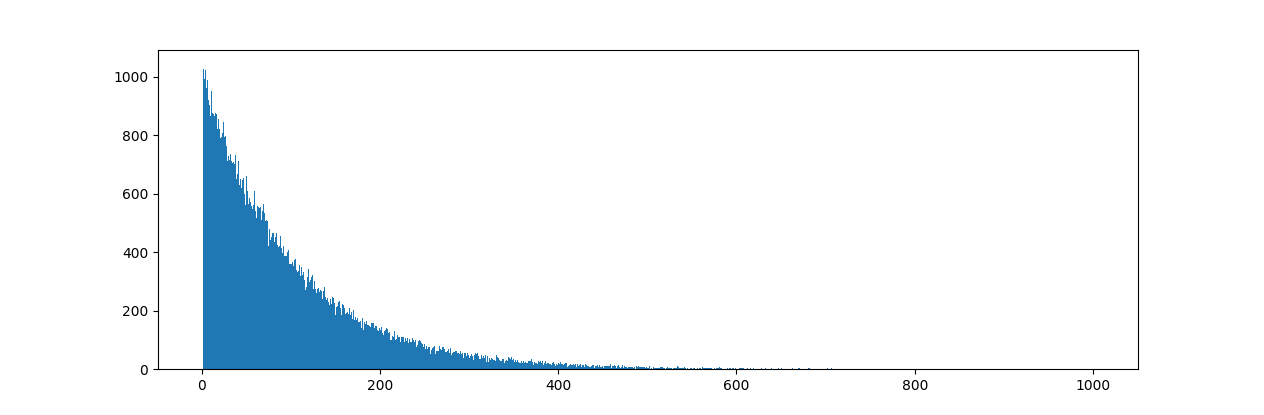
\includegraphics[width=0.8\textwidth]{a}
    \caption{Graph for 7a}
    \label{fig:a}
\end{figure}

\begin{figure}[htpb]
    \centering
    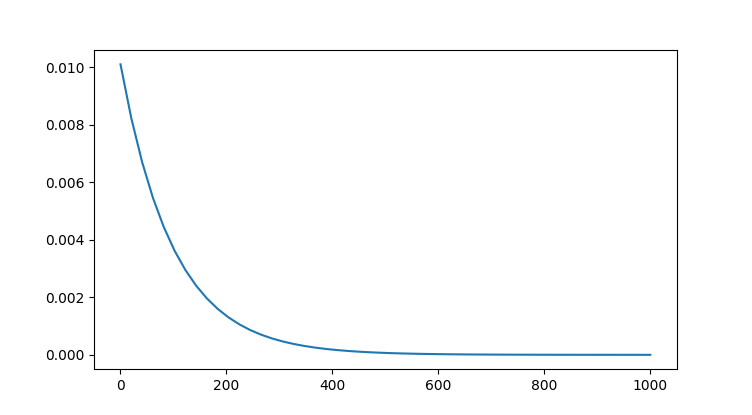
\includegraphics[width=0.8\textwidth]{b}
    \caption{Graph for 7b}
    \label{fig:b}
\end{figure}

\begin{figure}[htpb]
    \centering
    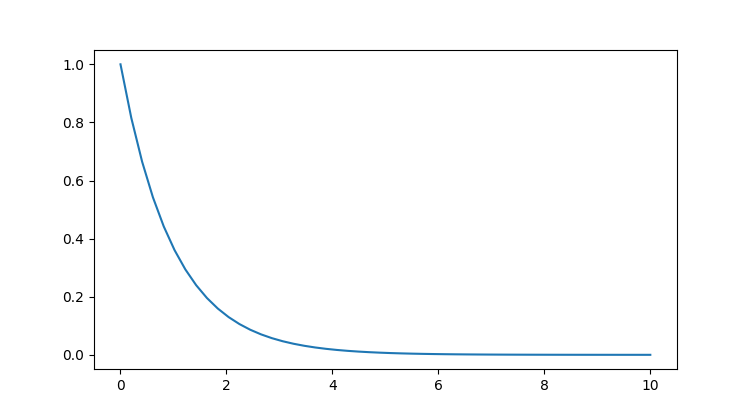
\includegraphics[width=0.8\textwidth]{c}
    \caption{Graph for 7c}
    \label{fig:c}
\end{figure}

\end{document}
